\documentclass[svgnames,11pt]{beamer}
\input{/home/tof/Documents/Cozy/latex-include/preambule_commun.tex}
\input{/home/tof/Documents/Cozy/latex-include/preambule_beamer.tex}
%\usepackage{pgfpages} \setbeameroption{show notes on second screen=left}
\author[]{Christophe Viroulaud}
\title{Principe d'un\\système d'exploitation\\Correction}
\date{\framebox{\textbf{ArchMat 08}}}
%\logo{}
\institute{Première - NSI}

\begin{document}
\begin{frame}
\titlepage
\end{frame}
\begin{frame}[fragile]
    \frametitle{}

    \begin{center}
        \begin{lstlisting}[language=Bash , basicstyle=\small, xleftmargin=2em, xrightmargin=2em]
MOV R0, #3
ADD R1,R0,#5
HALT
\end{lstlisting}
\captionof{code}{\centering Pour communiquer directement avec le processeur il faut utiliser un langage de bas-niveau.}
    \end{center}

\end{frame}
\begin{frame}
    \frametitle{}

    \begin{itemize}
        \item <1-> Chaque processeur accepte un langage différent.
        \item <2-> Chaque matériel (carte graphique, webcam, clavier\dots) possède des caractéristiques différentes.
    \end{itemize}

\end{frame}
\begin{frame}
    \frametitle{}

    \begin{aretenir}[]
    Pour réaliser un programme exécutable sur différentes machines et avec différents matériels, il faut créer une version pour chaque combinaison de périphériques.
    \\
    C'est une tâche énorme au vu de la multitude des matériels existants.
    \end{aretenir}

\end{frame}
\begin{frame}
    \frametitle{}

    \begin{framed}
        \centering Comment gérer les accès matériels de manière transparente?
    \end{framed}

\end{frame}
\section{Le système d'exploitation}
\begin{frame}
    \frametitle{Le système d'exploitation}
\begin{center}
    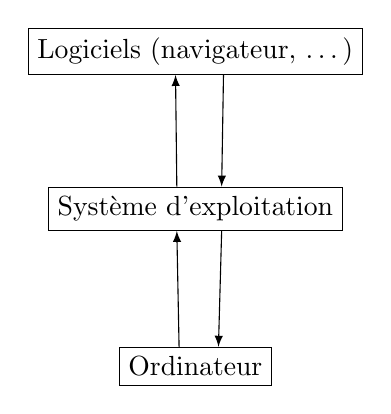
\begin{tikzpicture}
        \node[draw] (log) at(0,0) {Logiciels (navigateur, \dots)};
        \node[draw] (sys) at(0,-2) {Système d'exploitation};
        \node[draw] (mac) at(0,-4) {Ordinateur};
        \draw[->,>=latex] (log.-40) -- (sys.40);
        \draw[<-,>=latex] (log.-130) -- (sys.130);
        \draw[->,>=latex] (sys.-40) -- (mac.40);
        \draw[<-,>=latex] (sys.-130) -- (mac.130);
    \end{tikzpicture}
    \captionof{figure}{\centering Le système d'exploitation jour le rôle d'intermédiaire entre les programmes et la machine.}
\end{center}

\end{frame}
\begin{frame}
    \frametitle{}

    \begin{aretenir}[]
        \begin{itemize}
            \item Quand un programme doit utiliser un matériel, il demande l'accès au système d'exploitation.
            \item Le système d'exploitation utilise le \textbf{pilote (driver)} adapté pour contrôler le matériel en fonction de la demande du programme.
        \end{itemize}
    \end{aretenir}

\end{frame}
\begin{frame}
    \frametitle{}
Par exemple:
    \begin{itemize}
        \item<1-> Le navigateur \emph{Firefox} veut accéder à la webcam. Il demande l'accès au système d'exploitation.
        \item <2-> Le système d'exploitation repère la webcam et utilise le pilote adapté pour communiquer avec elle.
        \item <3-> Le flux vidéo de la webcam est récupéré par le système d'exploitation et envoyé au navigateur.
    \end{itemize}

\end{frame}
\section{Le système UNIX}
\begin{frame}
    \frametitle{Le système UNIX}
\begin{aretenir}[]
Le système UNIX est conçu à la fin des années 60. Il est écrit en langage C. Il est, plus tard, utilisé comme modèle pour construire d'autres systèmes d'exploitation:
\begin{itemize}
    \item Windows,
    \item Mac,
    \item Linux,
    \item BSD.
\end{itemize}
\end{aretenir}

\end{frame}
\begin{frame}
    \frametitle{}

    \begin{aretenir}[]
    Techniquement, \textbf{Linux} n'est pas un système d'exploitation. Il s'agit d'un \textbf{noyau (kernel)} qui gère les accès de bas-niveau (accès matériels, communication avec la mémoire, \dots)\\
    Grâce au noyau Linux, on peut construire un système d'exploitation GNU/Linux:
    \begin{itemize}
        \item Debian,
        \item Ubuntu,
        \item Fedora
        \item Mint.
    \end{itemize}
    \end{aretenir}

\end{frame}
\begin{frame}
    \frametitle{}

    \begin{aretenir}[]
    \begin{itemize}
        \item <1-> Les systèmes GNU/Linux sont \textbf{libres}: le code est ouvert et chacun peut, s'il le souhaite, modifier le contenu du système.
        \item <2-> Les systèmes Windows ou Mac sont \textbf{propriétaires}: il n'est pas possible de modifier le code du système.
    \end{itemize}
    \end{aretenir}

\end{frame}
\end{document}